%!TEX root = 497Notes-Temple.tex
\newpage
\section{Initialization for deep neural networks}
To build a machine learning algorithm, we need to define an architecture (e.g. Logistic regression, Support Vector Machine, Neural Network) and train it to learn parameters. The training of neural network is actually the iteration of the above architecture. Then, the initial guess of the parameters is important in avoiding gradient vanishing or blowup. 
The initialization step deals with the initial guess of parameters, and can be critical to the model's ultimate performance. 


\subsection{Xavier's Initialization with $\sigma  = id$}
The goal of Xavier initialization~\cite{glorot2010understanding} is to initialize the deep neural network to avoid gradient vanishing or blowup when the input is white noise. 


Recall the DNN models in Section \ref{sec:DNN}
\begin{equation}
\begin{cases}
f^1(x) &= W^1 x + b^1 \\
f^{\ell}(x) &= W^\ell \sigma(f^{\ell-1}(x)) + b^\ell \quad \ell = 2:L \\
f(x) &= f^{L} \\
\end{cases},
\end{equation}
with $x \in \mathbb{R}^{n_0}$ and $f^{\ell} \in \mathbb{R}^{n_\ell}$. More precisely, we have
\begin{equation}\label{key}
W^\ell \in \mathbb{R}^{n_{\ell} \times n_{\ell-1}}.
\end{equation}
We make the basic assumptions below:
\begin{itemize}
%% \item The input $x$ is a mean $0$ random variable with identity covariance, i.e. $\mathbb{E}(x) = 0$, $\mathbb{E}(x_ix_j) = 0$ if $i\neq j$, and $\mathbb{E}(x_i^2) = 1$
% \item \blue{The input $x$ is a mean $0$ random vector with the same variance for each component, i.e. $\mathbb{E}[[x]_i] = 0$ and $\mathbb{E}[[x]_i^2] (\mathbb{V} [[x]_i]) =$ $\mathbb{E}[[x]_j^2] (\mathbb{V}[[x]_j])$. }
% (Here we notice that, after data normalization as discussed before this assumption holds directly.)
 \item The initial weights $W^\ell_{ij}$ are i.i.d symmetric random variables with mean $0$, namely the 
 probability distribution of $W^\ell_{ij}$ is even.
 \item The initial bias $b^\ell = 0$.
\end{itemize}
The goal of Xavier's initialization is to ensure that the features $f^\ell$ and gradients do not blow up or vanish. Note that the mean of $f^\ell$ is zero, we only need to choose appropriate initial parameters to bound the variance of $f^\ell$. To this end we have the following lemma.

\begin{lemma}\label{lemm:init}
Under the previous assumptions $f^\ell_i$  is a symmetric random variable with $\mathbb{E}[f^\ell_i] = 0$.
Moreover, we have the following identity
\begin{equation}\label{eq:FWini}
\mathbb{V}[f^{\ell}_i] = \mathbb{E}[(f^{\ell}_i)^2] = \sum_{k}\mathbb{E}[(W^\ell_{ik})^2]\mathbb{E}[\sigma(f^{\ell-1}_k)^2].
\end{equation}
where the subscript $i$ of the notation $f_i^\ell$ represents the $i$-th component of $f^\ell$.
% \begin{equation}\label{key}
%  \mathbb V [f^{L}_i] =  \left(\Pi_{\ell=1}^{L} n_{\ell-1} {\rm Var} [W^\ell_{st}] \right)\mathbb V [x_j].
% \end{equation}
\end{lemma}
%Note that here we don't have that $f^\ell_i$ and $f^\ell_j$ are actually independent, just that they are `linearly' independent.
\begin{proof}
For general activation function $\sigma(x)$, let first prove that
$f^\ell_i$  is a symmetric random variable with $\mathbb{E}[f^\ell_i] = 0$.
For any $\ell$ and $1\le i \le n_\ell$, we have
\begin{equation}
 f^\ell_i = \sum_k W^\ell_{ik}\sigma(f^{\ell-1}_k) + b_i^\ell,
\end{equation}
Taking expectations, noting that $W^\ell_{ik}$ are independent of $f^{\ell-1}_k$ and that $b_i^\ell = 0$, we get
\begin{equation}
 \mathbb{E}[f^\ell_i] = \sum_k \mathbb{E}[W^\ell_{ik}]\mathbb{E}[\sigma(f^{\ell-1}_k)] = 0.
\end{equation}
since $\mathbb{E}[W^\ell_{ik}] = 0$.
Moreover, if the $W_{ij}^\ell$ are symmetric, it is clear that $f^\ell_i$ will be.

 
% Furthermore, we calculate (note that $b^\ell = 0$)
% \begin{equation}
% \begin{split}
%  \mathbb{E}(f^\ell_if^\ell_j) &= \mathbb{E}\left(\left(\sum_k W^\ell_{ik}\sigma(f^{\ell-1}_k)\right)\left(\sum_l W^\ell_{jl}\sigma(f^{\ell-1}_l)\right)\right) \\ &= \sum_{k,l}\mathbb{E}(W^\ell_{ik}W^\ell_{jl}\sigma(f^{\ell-1}_k)\sigma(f^{\ell-1}_l))
%  \end{split}
% \end{equation}
%
%Since $W^\ell_{ik}$ and $W^\ell_{jl}$ are independent ($i\neq j$), and are both independent of $f^{\ell-1}$, each of the terms above is 
%\begin{equation}
% \mathbb{E}(W^\ell_{ik})\mathbb{E}(W^\ell_{jl})\mathbb{E}(\sigma(f^{\ell-1}_k)\sigma(f^{\ell-1}_l)) = 0.
%\end{equation}
Next we calculate the variance of $f^{\ell}_i$, we get
\begin{equation}
\begin{split}
 \mathbb{V}[f^{\ell}_i] = \mathbb{E}[(f^{\ell}_i)^2] &= \mathbb{E}\left[\left(\sum_k W^\ell_{ik}\sigma(f^{\ell-1}_k)\right)\left(\sum_l W^\ell_{il}\sigma(f^{\ell-1}_l)\right)\right]\\ &= \sum_{k,l}\mathbb{E}[W^\ell_{ik}W^\ell_{il}\sigma(f^{\ell-1}_k)\sigma(f^{\ell-1}_l)].
 \end{split}
\end{equation}
In the above sum we will have $W^\ell_{ik}$ and $W^\ell_{il}$ independent unless $k = l$. In this case the term will be $0$. So the only terms which remain are those for which $k=l$ and we get
\begin{equation}\label{eq:FWini}
  \mathbb{E}[(f^{\ell}_i)^2] = \sum_{k}\mathbb{E}[(W^\ell_{ik})^2]\mathbb{E}[\sigma(f^{\ell-1}_k)^2].
\end{equation}

\end{proof}


Now, we assume $\sigma  = id$. This assumption is pretty reasonably since most activation functions in use at the time (such as the hyperbolic tangent) were close to the identity near $0$. 

\begin{lemma}\label{th:idnormal}
If $\sigma  = id$, 
 \begin{equation}\label{key}
	\mathbb V [f^{L}_i] =  \left(\Pi_{\ell=2}^{L} n_{\ell-1} {\rm Var} [W^\ell_{st}] \right) \left(\mathbb{V}[W^1_{st}]\sum_{j}\mathbb{E}[( x^j)^2] \right),
	\end{equation}
where $x^j$ represents the $j$-th component of data $x$.
\end{lemma}
\begin{proof}
Let us prove it this by induction. For $\ell=1$,
\begin{equation}\label{key}
\mathbb{V}[f^{1}_i] = \sum_{j}\mathbb{E}[(W^1_{ij})^2]\mathbb{E}[( x^j)^2] = {\mathbb{E}[(W^1_{ij})^2]  \left(\sum_{j}\mathbb{E}[( x^j)^2] \right)},
\end{equation}
for any $i = 1,2,\cdots, n_1$. Since we already know that
	\begin{equation}\label{key}
	\mathbb{V}[f^1_i ] = {\mathbb{E}[(W^1_{ij})^2]  \left(\sum_{j}\mathbb{E}[( x^j)^2] \right)} = \mathbb{V}[f^1_k], \quad \forall i,k,
	\end{equation}
	from derivation in $\ell=1$. We will see that for $\ell=2$,
	\begin{equation}\label{key}
	\mathbb{V}[f^2_i ] = n_1 \mathbb{V}[W^2_{ij}]  \mathbb{V}[ f^1_j] = n_1     \mathbb{V}[W^2_{st}] \left(\mathbb{V}[W^1_{st}]\sum_{j}\mathbb{E}[(x^j)^2] \right).
	\end{equation}
By induction, 
\begin{equation}\label{key}
	\mathbb V [f^{L}_i] =  \left(\Pi_{\ell=2}^{L} n_{\ell-1} {\rm Var} [W^\ell_{st}] \right) \left(\mathbb{V}[W^1_{st}]\sum_{j}\mathbb{E}[( x^j)^2] \right).
	\end{equation}
\end{proof}
%We will see in the next section that (as first observed by Kaiming He) if $\sigma$ is the ReLU function, 
%then we don't need to make this assumption since the left hand side in \eqref{eq:FWini} can be calculated exactly. 

According to Theorem \ref{th:idnormal}, one way to make sure the variance $\mathbb{V}[W^\ell_{ik}]$ does not blow up is to set 
\begin{equation}\label{varianceW}
\mathbb{V}[W^\ell_{ik}] = \frac{1}{n_{\ell-1}}, \quad \forall \ell \ge 2.
\end{equation}
In this case,
\begin{equation}
\mathbb V [f^{L}_i] = \mathbb V [f^{L-1}_j] = \cdots =  \mathbb V [f^{1}_k] = \mathbb{V}[W^1_{st}]\sum_{j}\mathbb{E}[(x^j)^2].
\end{equation}
Thus, in pure DNN models, it is enough to just control $\displaystyle \sum_{j}\mathbb{E}[(x^j)^2]$.
The choice \eqref{varianceW} comes from the analysis of $\mathbb{V}[W^\ell_{ik}]$. We can also consider the propagation of the gradient $\frac{\partial L(\theta)}{\partial f^\ell}$. A similar analysis suggests the choice 
$
\mathbb{V}[W^\ell_{ik}] = \frac{1}{n_{\ell}}.
$
Thus, the {\bf Xavier's initialization} suggests to initialize $W^\ell_{ik}$ with variance as:
\begin{itemize}
	\item To control $\mathbb V [f^{\ell}_i] $:
	\begin{equation}\label{key}
	{\rm Var}[W^\ell_{ik}] = \frac{1}{n_{\ell-1}}.
	\end{equation}
	\item To control $\mathbb{V}[\frac{\partial L(\theta)}{\partial f_i^\ell}]$:
	\begin{equation}\label{key}
	{\rm Var}[W^\ell_{ik}] = \frac{1}{n_{\ell}}.
	\end{equation}
	\item Trade-off to control $\mathbb{V} [\frac{\partial L(\theta)}{\partial W_{ik}^\ell}]$: 
	\begin{equation}\label{key}
	{\rm Var}[W^\ell_{ik}] = \frac{2}{n_{\ell-1} + n_\ell}.
	\end{equation}
\end{itemize}
Here we note that, this analysis works for all symmetric type distribution around zero. We often just choose uniform distribution $\mathcal U(-a,a)$ and normal distribution $\mathcal N(0,s^2)$. Since the expectation of $W^{\ell}_{ik}$ is zero and the variance is given above, the final version of Xavier's initialization takes the trade-off type as
\begin{equation}
W^{\ell}_{ik} \sim \mathcal{U}(-\sqrt{\frac{6}{n_\ell+n_{\ell-1}}}, \sqrt{\frac{6}{n_\ell+n_{\ell-1}}}),\quad \text{ or }\quad
W^{\ell}_{ik} \sim \mathcal{N}(0,  {\frac{2}{n_\ell+n_{\ell-1}}}).
\end{equation}


%%%%%%%%%%%%%%%%%%%%%%%%%%%%%%
\subsection{Variance analysis in backward propagation phase}
Recall the loss function
$$
L(\theta)=\mathbb{E}_{(x, y) \sim D} \ell \left(\operatorname{softmax}\left(f^{L}\right), y\right),
$$
where $ f^{L}(x; \theta) $  is the DNN function defined by 
$$
\left\{\begin{array}{l}f^{1}(x)=W^{1} x+b^{1} \\ f^{l}(x)=W^{l} \sigma\left(f^{l-1}(x)\right)+b^{l} \quad \forall l=2, \cdots L\end{array}\right. .
$$
Then we have the following backward propagation ("BP") formula
$
\frac{\partial L(\theta)}{\partial W^{l}}=\frac{\partial L}{\partial f^{l}} \cdot \frac{\partial f^{l}}{\partial W^{l}},
$
where 
$\frac{\partial L}{\partial t^{l}} \in \mathbb{R}^{n_e}, \frac{\partial f}{\partial W^{l}} \in \mathbb{R}^{n_{e} \times\left(n_{e} \times n_{e-1}\right)}$. More Precisely,
$$
\frac{\partial L(\theta)}{\partial W_{s t}^{l}}=\sum\limits_{i=1}^{n_{l}}\left(\frac{\partial L(\theta)}{\partial f_{i}^{l}} \cdot \frac{\partial f_{i}^{l}}{\partial W_{s t}^{l}}\right).
$$
Assume that
\begin{enumerate}
\item $\left\{\frac{\partial L(\theta)}{\partial f_{i}^{l}} \cdot \frac{\partial f_{i}^{l}}{\partial W_{s t}^{L}}\right\}_{i=1}^{n_{e}}$ are independent
\item For each i,   $ \frac{\partial L(\theta)}{\partial f_{i}^{l}}  $ and $\frac{\partial f_{i}^{l}}{\partial W_{s t}^{l}}$ are independent 
\end{enumerate}
Actually, we can not such make general assumptions as $L(\theta), f_{i}^{l}, \frac{\partial f_{i}^{l}}{\partial W_{st}} \frac{\partial L(\theta)}{\partial f_{i}^{l}}$   are all fixed. We still make these assumption here to get some idea of the choice of $W_{s t}^{l}$. 
\begin{lemma}\label{th:idnormal2}
If $\sigma =id$ and  the above assumption holds,
$$\mathbb{V}\left[\frac{\partial L (\theta)}{\partial W_{s t}^{l}}\right] = \prod\limits_{j=l+1}^{L-1} n_{j} \mathbb{V}\left[W_{s t}^{j}\right] \left(\mathbb{V}\left[W_{s t}^{L}\right]\sum\limits_{k=1}^{n_{L}} \mathbb{E}\left[\left(\frac{\partial L(\theta)}{\partial f_{k}^{2}}\right)^{2}\right]\right) 
\prod\limits_{j=2}^{l-1} n_{j} \mathbb{V}\left[W_{s t}^{j}\right] \left(\mathbb{V}\left[W_{s t}^{1}\right]\sum\limits_{R=1}^{d} \mathbb{E}\left[ X_{k}^{2}\right]\right).
$$
\end{lemma}
\begin{proof}
The assumption leads to
\begin{equation}\label{normale0}
\mathbb{V}\left[\frac{\partial L(\theta)}{\partial W_{st}^{l}}\right]=\sum\limits_{i=1}^{n_{l}}\left( \mathbb{E}\left[\left(\frac{\partial L(\theta)}{\partial f^{l}_{i}}\right)^{2}\right] \mathbb{E}\left[\left(\frac{\partial f_{i}^{l}}{\partial W_{s t}^{l}}\right)^{2}\right] - \left(\mathbb{E}\left[\frac{\partial L(\theta)}{\partial f_{i}^{l}}\right] \mathbb{E}\left[\frac{\partial f_{i}^{l}}{\partial W_{s t}^{l}}\right]\right)^{2}\right) .
\end{equation}
This implies that we only need to consider $ \mathbb{E}\left[\left(\frac{\partial L(\theta)}{\partial f_{i}^{l}}\right)^{2}\right] $ and  $ \mathbb{E}\left[\left(\frac{\partial f_{i}^{l}}{\partial W_{s t}^{l}}\right)^{2}\right]$.
\begin{enumerate}
\item Consider $ \mathbb{E}\left[\left(\frac{\partial L(\theta)}{\partial f_{i}^{l}}\right)^{2}\right] $. By chain rule:
	$$
	\begin{aligned} 
	\frac{\partial L(\theta)}{\partial f_{i}^{l}} &=\frac{\partial L(\theta)}{\partial f^{l+1}}\cdot \frac{\partial f^{l+1}}{\partial f_{i}^{l}} =\sum_{j=1}^{n_{l+1}} \frac{\partial L(\theta)}{\partial f_{j}^{l+1}} \frac{\partial f_{j}^{l+1}}{\partial f_{i}^{l}}
	 \\ &=\sum_{j=1}^{n_{l+1}} W_{j i}^{l+1} \sigma^{\prime}\left(f_{i}^{l}\right) \frac{\partial L(\theta)}{\partial f_{j}^{l+1}}=\sum\limits_{j=1}^{n_{l+1}} W_{j i}^{l+1} \frac{\partial L(\theta)}{\partial f_{j}^{l+1}}(\mbox{ if }\sigma=id)
	\end{aligned} 
	$$
	Keep doing this:
	$$
	\frac{\partial L(\theta)}{\partial f^{l}}=\left[W^{l+1}\right]^{\top} \cdot\left[W^{l+2}\right]^{\top} \cdots\left[W^{L}\right]^{T} \frac{\partial L(\theta)}{\partial f^{L}}
	$$
	Assume the independence of $ \frac{\partial L(\theta)}{\partial f^{L}} $  with $W^{l+i}, i= 1,2, \dots$.
	( Still we make this assumption although this can not be ture, as $ \frac{\partial L(\theta)}{\partial f^{l}} $ contains  $W^{l+i}$.) Then 
	$$
	\mathbb{E}\left[\frac{\partial L(\theta)}{\partial f_{i}^{l}}\right]=\sum\limits_{j} \mathbb{E}\left[W_{j i}^{l+1}\right] \mathbb{E}\left[\frac{\partial L(\theta)}{\partial f_{j}^{l }}\right]=0
	$$
	\begin{equation}\label{normale1}
	\mathbb{E}\left[\left(\frac{\partial L(\theta)}{\partial f_{i}^{l}}\right)^{2}\right]=\mathbb{V}\left[{\frac{\partial L(\theta)}{\partial f_{i}^{l}}}\right]=\prod\limits_{j=l+1}^{L-1} n_{j} \mathbb{V}\left[W_{s t}^{j}\right] \cdot\left(\mathbb{V}\left[W_{s t}^{L}\right] \sum\limits_{i=1}^{n_{L}} \mathbb{E}\left[\left(\frac{\partial L( \theta)}{\partial f_{i}^{L}}\right)^{2}\right]\right)
	\end{equation}
    \item Consider $ \mathbb{E}\left[\left(\frac{\partial f_{i}^{l}}{\partial W_{s t}^{l}}\right)^{2}\right]
    $. By definition, 
    $
    \frac{\partial f_{i}^{l}}{\partial W_{s t}^{l}}=\delta_{i s} \sigma\left(f_{t}^{l-1}\right)
    $
    namely, only
	$
	\frac{\partial f_{s}^{l}}{\partial W_{s t}^{l}} \not = 0,
	$
	and $\frac{\partial f_{s}^{l}}{\partial W_{s t}^{l}} = \sigma\left(f^{l-1}_{t}\right)$. If $ \sigma $=id, apply the forward results
		\begin{enumerate}
		\item Expectation: 
		$$
		\mathbb{E}\left[\left(\frac{\partial f_{s}^{l}}{\partial W_{s t}^{l}}\right)\right]=0.
		$$
		\item Variance:
		\begin{equation}\label{normale2}
		\begin{split}
		\mathbb{E}\left[\left(\frac{\partial f_{s}^{l}}{\partial W_{s t}^{l}}\right)^{2}\right]& =\mathbb{E}\left[\left(f_{t}^{l-1}\right)^{2}\right]=\mathbb{V}\left[ f_{t}^{l-1}\right]
		\\
		&=\prod\limits_{j=2}^{l-1} n_{j-1} \mathbb{V}\left[W_{s t}^{j}\right] \cdot\left(\mathbb{V}\left[W_{s t}^{1}\right] \sum\limits_{k=1}^{d} \mathbb{E}\left[X_k^{2}\right]\right).
		\end{split}
		\end{equation}
		\end{enumerate} 
\end{enumerate}
A combination of \eqref{normale0}, \eqref{normale1} and \eqref{normale2} completes the proof.
\end{proof}

Next we consider $ \mathbb{V}\left[\frac{\partial L(\theta)}{\partial W^{l} _{st}}\right] $.
	\begin{equation*}
	\begin{split} 
	&\mathbb{V}\left[\frac{\partial L(\theta)}{\partial W^{l} _{st}}\right] =\mathbb{V}\left[\frac{\partial L (\theta)}{\partial f_{s}^{l}}\right] \cdot \mathbb{V}\left[f^{l-1}_{t}\right] 
	\\
	 =& \prod\limits_{j=l+1}^{L-1} n_{j} \mathbb{V}\left[W_{s t}^{j}\right] \left(\mathbb{V}\left[W_{s t}^{L}\right]\sum\limits_{k=1}^{n_{L}} \mathbb{E}\left[\left(\frac{\partial L(\theta)}{\partial f_{k}^{L}}\right)^{2}\right]\right) \times \prod\limits_{j=2}^{l-1} n_{j} V\left[W_{s t}^{j}\right] \left(\mathbb{V}\left[W_{s t}^{1}\right]\sum\limits_{R=1}^{d} \mathbb{E}\left[ X_{k}^{2}\right]\right),
	\end{split}
	\end{equation*}
	where $ \mathbb{V}_{1}=\left(\mathbb{V}\left[W_{s t}^{1}\right]\sum\limits_{k=1}^{d} \mathbb{E}\left[ X_{k}^{2}\right]\right)	$,
$  \mathbb{V}_{L}=\mathbb{V}\left[W_{s t}^{L}\right]\sum\limits_{k=1}^{n_{L}} \mathbb{E}\left[ (\frac{\partial L(\theta)}{\partial f_{k}^{L}})^{2}\right]$.


We consider
$$
	\mathbb{V}\left[W_{s t}^{l}\right]=f\left(n_{l}, n_{l-1}\right).
	$$
 We summarize Lemma \ref{th:idnormal} and Lemma \ref{th:idnormal2} as below
 \begin{enumerate}
\item 
$ 
\mathbb{V}\left[f_{i}^{l}\right]  =\prod\limits_{j=2}^{l} n_{j-1} f\left(n_{j}, n_{j-1}\right)\left(\mathbb{V}\left[W_{s t}^{1}\right]\sum\limits_{k=1}^{d} \mathbb{E}\left[ X_{k}^{2}\right]\right) 
$
\item $\mathbb{V}\left[\frac{\partial L(\theta)}{\partial f_{i}^{2}}\right]= \prod\limits_{j=1+1}^{L-1} n_{j} f\left(n_{j}, n_{j-1}\right)\cdot\left(\mathbb{V}\left[W_{s t}^{L}\right] \sum\limits_{i=1}^{n_{L}} \mathbb{E}\left[\left(\frac{\partial L( \theta)}{\partial f_{i}^{l}}\right)^{2}\right]\right) 
$
\item $ \mathbb{V}\left[\frac{\partial L(\theta)}{\partial W^{l} _{st}}\right] = \prod\limits_{j=l+1}^{L-1}n_{j} \cdot f\left(n_{j}, n_{j-1}\right) \cdot \prod\limits_{j=2}^{l-1}n_{j-1}f\left(n_{j}, n_{j-1}\right) \times \mathbb{V}_{1} \times \mathbb{V}_{L}
$
\end{enumerate}
Based on the equations above, we have different choice of $\mathbb{V}\left[W_{s t}^{l}\right]$
\begin{enumerate}
	\item If $f\left(n_{1}, n_{j-1}\right)=\frac{1}{n_{j-1}}$ (control $W[f_{i}^{l}]$), 
	$\mathbb{V}\left[\frac{\partial L(\theta)}{\partial W_{s t}^{l}}\right]$ will decrease as $l$ grow up. (Notice that $n_{l}>n_{k}$ if $l>k$)
	\item If $f\left(n_{j}, n_{j-1}\right)=\frac{1}{n_{j}}$ (control $V[\frac{\partial L(\theta)}{ \partial f_{i}^{L}} ]$),
	$
	\mathbb{V}\left[\frac{\partial L(\theta)}{\partial W_{s t}^{l}}\right]$	
	 still decrease!
	\item If $f\left(n_{j}, n_{j-1}\right)=\frac{2}{n_{j}+n_{j-1}}( \leq \frac{1}{\sqrt{n_{j} n_{j-1}}})$,
	$
	\mathbb{V}\left[\frac{\partial L (\theta)}{\partial W^{l}_{st}}\right]=\frac{\sqrt{n_{L-1}} \cdot \sqrt{n_{1}}}{\sqrt{n_{l}} \cdot \sqrt{n_{l-1}}} \times \mathbb{V}_{1} \times \mathbb{V}_{L}
	$
	decrease!
\end{enumerate}
	
\paragraph{Question}
Can we design some other choices of  $ \mathbb{V}\left[ W^{l} _{st}\right]$ such  that  $\mathbb{V} \left[\frac{\partial L(\theta)}{\partial W^{l} _{st}}\right]$ admits the following properties:
\begin{itemize}
	\item Keep constant,
	\item Increase,
	\item Change with certain scale.
\end{itemize}
%%%%%%%%%%%%%%%%%%%%%%%%%%%%%%
%See the separate file in {``6DL/HandWrittenNotes/InitBackward.pdf''}
%\includepdf[pages=-,pagecommand={}]{HandWrittenNotes/InitBackward.pdf}
%\includepdf[pages=-,pagecommand={}]{497/handwritten_notes/MultidimensionalVariance.pdf}


\subsection{Kaiming's initialization}
In~\cite{he2015delving}, Kaiming He and others extended this analysis to get an \textit{exact} result when the activation function is the  ReLU.

We first have the following lemma for symmetric distribution.
\begin{lemma}
	If $X_i \in \mathbb{R}$ for $i=1:n$ are i.i.d with symmetric probability density function $p(x)$, i.e. $p(x)$ is even.
	Then for any nonzero random vector $Y = (Y_1, Y_2, \cdots, Y_n) \in \mathbb{R}^n$ which is independent with $X_i$, 
	the following random variable
	\begin{equation}\label{key}
	Z = \sum_{i=1}^n X_i Y_i,
	\end{equation} 
	is also symmetric.
\end{lemma}

\begin{proof}
	Let us denote the joint distribution function for $Y$ as $q(y_1, \cdots, y_n)$. Then
	the joint distribution density function for $(X,Y)$ is 
	\begin{equation}\label{key}
	f(x_1, \cdots, x_n,y_1, \cdots, y_n) = p(x_1)p(x_2)\cdots p(x_n)q(y_1, y_2, \cdots, y_n).
	\end{equation}
	Then we have the following probability function
	\begin{equation}\label{key}
	\begin{aligned}
	\mathbb P(Z < z) &= \int_{\sum_{i=1}^n {x_i y_i} < z} f(x_1, \cdots, x_n,y_1, \cdots, y_n)  dxdy \\
	&= \int_{\sum_{i=1}^n {x_i y_i} < z} p(x_1)p(x_2)\cdots p(x_n)q(y_1, y_2, \cdots, y_n)  dxdy \\
	&= \int_{\sum_{i=1}^n {-x_i y_i} > -z} p(x_1)p(x_2)\cdots p(x_n)q(y_1, y_2, \cdots, y_n)  dxdy\\
	&= \int_{\sum_{i=1}^n {-x_i y_i} > -z} p(-x_1)p(-x_2)\cdots p(-x_n)q(y_1, y_2, \cdots, y_n)  dxdy\\
	&= \int_{\sum_{i=1}^n \tilde x_i y_i >-z} p(\tilde x_1)p(\tilde x_2)\cdots p(\tilde x_n)q(y_1, y_2, \cdots, y_n)  d\tilde xdy\\
	&= \mathbb P(Z >- z).
	\end{aligned}
	\end{equation}
\end{proof}

Then state the following result for ReLU function and random variable with 
symmetric distribution around $0$.
\begin{lemma}
If $X$ is a random variable on $\mathbb{R}$ with symmetric probability density $p(x)$ around zero, i.e., 
\begin{equation}\label{key}
p(x) = p(-x).
\end{equation}
Then we have $\mathbb{E} X = 0$ and 
\begin{equation}\label{key}
\mathbb{E}[[{\rm ReLU}(X)]^2] = \frac{1}{2}{\rm Var}[X].
\end{equation}
\end{lemma}
\begin{proof}
	By definition
	\begin{equation}\label{key}
	\mathbb{E} X = \int_{-\infty}^\infty xp(x)d(x) = 0. \quad (\text{since } p(x) = p(-x)).
	\end{equation}
	Furthermore, 
	\begin{equation}\label{key}
	\begin{aligned}
	\mathbb{E}[[{\rm ReLU}(X)]^2] &= \int_{-\infty}^\infty ({\rm ReLU}(x))^2 p(x)  dx \\
	&= \int_{0}^\infty x^2 p(x) dx \\
	&= \frac{1}{2} \int_{-\infty}^\infty (x - \mathbb E [x])^{2} p(x) dx \\
	& = \frac{1}{2} \mathbb E[ [X - \mathbb{E} X]^2] \\
	& = \frac{1}{2}\mathbb{V}[X].
	\end{aligned}
	\end{equation}
\end{proof}



Based on the previous Lemma~\ref{lemm:init}, we know that $f^{\ell-1}_k$ is a symmetric distribution around $0$.
The most important observation in Kaiming's paper~\cite{he2015delving} is that:
\begin{equation*}\label{key}
\mathbb{V}[ f^\ell_i ] = n_{\ell-1}  \mathbb{V}[W^\ell_{ij}] {\mathbb{E}[[\sigma(f^{\ell-1}_j)]^2]} = n_{\ell-1} \mathbb{V}[W^\ell_{ik}] {\frac{1}{2} \mathbb{V}[f^{\ell-1}_k]},
\end{equation*}
{if $\sigma = {\rm ReLU}$}.
Thus, Kaiming's initialization suggests to take:
\begin{equation}\label{key}
\mathbb{V}[W^\ell_{ik}] = \frac{2}{n_{\ell-1}}, , \quad \forall \ell \ge 2.
\end{equation}

For the first layer $\ell=1$, by definition
\begin{equation}\label{key}
f^1 = W^1 x + b^1,
\end{equation}
there is no ReLU, thus it should be $\mathbb{V}[W^1_{ik}] = \frac{1}{d}$. 
For simplicity, they still use $\mathbb{V}[W^1_{ik}] = \frac{2}{d}$ in the paper~\cite{he2015delving}. Similarly, an analysis of the propagation of the gradient suggests that we set 
\begin{equation}\label{key}
\mathbb{V}[W^\ell_{ik}] = \frac{2}{n_{\ell}}.
\end{equation}
However, in paper~\cite{he2015delving} authors did not suggest to take the trade-off version, they just chose 
\begin{equation}\label{key}
\mathbb{V}[W^\ell_{ik}] = \frac{2}{n_{\ell-1}},
\end{equation} as default.
Thus, the final version of Kaiming's initialization takes the forward type as
\begin{equation}
W^{\ell}_{ik} \sim \mathcal{U}(-\sqrt{\frac{6}{n_{\ell-1}}}, \sqrt{\frac{6}{n_{\ell-1}}}),
\quad\text{ or }\quad
W^{\ell}_{ik} \sim \mathcal{N}(0,  {\frac{2}{n_{\ell-1}}}).
\end{equation}

%And another difference is that Xavier use the uniform distribution but He use the Gaussian distribution. 
%More precisely, 
%However, in Pytorch implementation, the uniform distribution is also applied.


\section{Data normalization in CNNs}
For CNN models, following the analysis above we have the next iterative scheme in CNNs
\begin{equation}\label{key}
f^{\ell,\nu} = K^{\ell,\nu} \ast \sigma (f^{\ell,\nu-1}),
\end{equation}
where the previous step $f^{\ell,\nu-1} \in \mathbb{R}^{c_\ell\times n_\ell \times m_\ell }$, the current step $f^{\ell,\nu} \in \mathbb{R}^{h_\ell\times n_\ell \times m_\ell}$ and $K \in \mathbb{R}^{(2k+1) \times (2k+1) \times h_\ell \times c_\ell}$.
Thus we have
\begin{equation}\label{key}
f^{\ell,\nu}_{h;p,q} = \sum_{c=1}^{c_\ell}\sum_{s,t=-k}^k K^{\ell,\nu}_{h,c;s,t} \ast \sigma (f^{\ell,\nu-1}_{c;p+s,q+t}).
\end{equation}
Take variance on both sides, we will get
\begin{equation}\label{key}
\mathbb{V} [f^{\ell,\nu}_{h;p,q}] = c_\ell (2k+1)^2 \mathbb{V}[K^{\ell,\nu}_{h,o;s,t}] \mathbb{E}[(f^{\ell,\nu-1}_{o;p+s,q+t})^2],
\end{equation}
thus we have the following initialization strategies:
\begin{description}
	\item[Xavier's initialization] 
	\begin{equation}\label{key}
	\mathbb{V}[K^{\ell,\nu}_{h,o;s,t}] = \frac{2}{ (c_\ell + h_\ell) (2k+1)^2}.
	\end{equation}
	\item[Kaiming's initialization]
	\begin{equation}\label{key}
	\mathbb{V}[K^{\ell,\nu}_{h,o;s,t}] = \frac{2}{c_\ell (2k+1)^2}.
	\end{equation}
\end{description}

Here we can take this Kaiming's initialization as:
\begin{itemize}
	\item Double the Xavier's choice, and get
	\begin{equation}\label{key}
	\mathbb{V}[K^{\ell,\nu}_{h,o;s,t}] = \frac{4}{(c_\ell + h_\ell )(2k+1)^2}.
\end{equation}
	\item Then pick $c_\ell$ or $h_\ell$ for final result  
	\begin{equation}\label{key}
	\mathbb{V}[K^{\ell,\nu}_{h,o;s,t}] = \frac{2}{c_\ell (2k+1)^2}.
	\end{equation}
\end{itemize}

And they have the both uniform and normal distribution type.
\begin{figure}[H]
	\begin{center}
		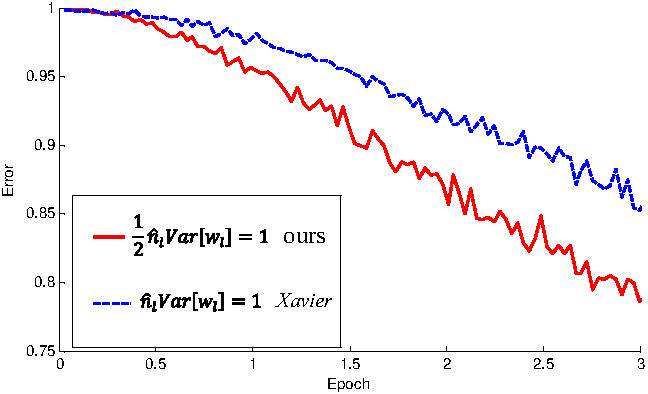
\includegraphics[width=0.45\linewidth]{converge_22layers}
	\end{center}
	\caption{The convergence of a \textbf{22-layer} large model. The $x$-axis is the number of training epochs. The y-axis is the top-1 error of 3,000 random val samples, evaluated on the center crop. Use ReLU as the activation for both cases. Both Kaiming's initialization (red) and ``\emph{Xavier's}'' (blue) \cite{glorot2010understanding} lead to convergence, but Kaiming's initialization starts reducing error earlier.}
	\label{fig:converge_22layers}
\end{figure}
\begin{figure}[H]
	\begin{center}
		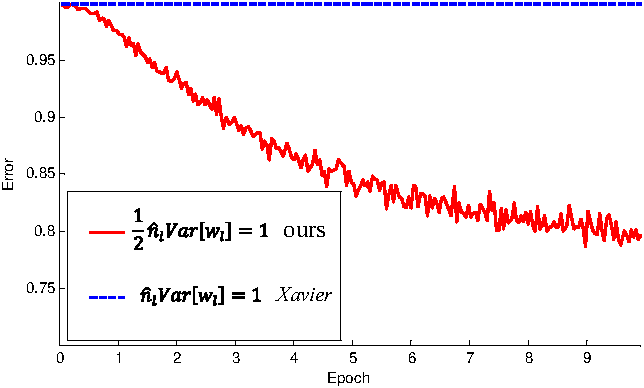
\includegraphics[width=0.5\linewidth]{converge_30layers}
	\end{center}
	\caption{The convergence of a \textbf{30-layer} small model (see the main text). Use ReLU as the activation for both cases. Kaiming's initialization (red) is able to make it converge. But ``\emph{Xavier's}'' (blue) \cite{glorot2010understanding} completely stalls - It is also verified that that its gradients are all diminishing. It does not converge even given more epochs.}
	\label{fig:converge_30layers}
\end{figure}

Given a 22-layer model, in Cifar10 both Kaiming's and Xavier's initialization are able to converge and the validation accuracies with two different initialization 
are about the same(error is 33.82,33.90). But the convergence with Kaiming's initialization is faster than Xavier's.
With extremely deep model with up to 30 layers, 
Kaiming's initialization is able to make the model convergence. On the contrary, Xavier's method completely stalls the learning.


\endinput

\iffalse
\subsection{Basic assumptions in Xavier's and Kaiming's initialization.}
\begin{itemize}
	\item $f^\ell$ is a random vector and $f^\ell_i$ for $i = 1:n_\ell$ are i.i.d.
	\item $W^\ell$ should be initialized as random vector independently to $f^{\ell-1}$ and $W^\ell_{ij}$ 
	for all $i = 1:n_{\ell},j=1:n_{\ell-1}$ are i.i.d with a zero mean and symmetric distribution around zero.
	\item $b^\ell = 0$.
\end{itemize}


\subsection{Xavier's initialization.} There are two steps in Xavier's initialization:
\begin{itemize}
	\item forward variance formula,
	\item backward variance formula.
\end{itemize}
For forward variance:
\begin{equation}\label{key}
f^\ell_i = W^\ell_i \cdot \sigma(f^{\ell-1}) + b^\ell_i.
\end{equation}
Take variance on both sides:
\begin{equation}\label{key}
{\rm Var}[ f^\ell_i ] = {\rm Var}[W^\ell_i \cdot \sigma(f^{\ell-1})]+ b^\ell _i].
\end{equation}
They further \red{assume that $\sigma  = id$} and
\begin{equation}\label{key}
\mathbb{E}[ f^{\ell-1}_j] = 0.
\end{equation}
Then, they have
\begin{equation}\label{key}
{\rm Var}[ f^\ell_i ]  = n_{\ell-1}{\rm Var}[W^\ell_{ij}] {\rm Var}[f^{\ell-1}_j], 
\end{equation}
for all $i=1:n_\ell$ and $j = 1:n_{\ell-1}$.
This leads to
\begin{equation}\label{key}
{\rm Var}[ f^L_i ]  = {\rm Var}[f^{0}_j] (\prod_{\ell=1}^L n_{\ell-1}{\rm Var}[W^\ell_{st}] ),
\end{equation}
for any $i,j,s,t$.
The ideal situation to control the variance of $f^{\ell}$ during forward propagation is that
\begin{equation}\label{key}
{\rm Var}[ f^L_i ] =  {\rm Var}[f^{0}_j].
\end{equation}
Thus, a sufficient condition from forward analysis is:
\begin{equation}\label{key}
{\rm Var}[W^\ell_{ij}] = \frac{1}{n_{\ell-1}}.
\end{equation}

The so-called backward variance analysis is to investigate the variance of $\frac{\partial L(\theta)}{\partial f^\ell}$ and $\frac{\partial L(\theta)}{\partial f^{\ell-1}}$
where $L(\theta)$ is the loss function.
This is important because that:
\begin{equation}\label{key}
\frac{\partial L(\theta)}{\partial f^{\ell-1}} = \frac{\partial L(\theta)}{\partial f^\ell} \frac{\partial f^\ell}{\partial f^{\ell-1}}.
\end{equation}
We have the next backward propagation case:
\begin{equation}\label{key}
\frac{\partial L(\theta)}{\partial f^{\ell-1}} = [W^\ell]^T \cdot \frac{\partial L(\theta)}{\partial f^\ell}.
\end{equation}
Similarly, we can derive the condition to keep 
\begin{equation}\label{key}
{\rm Var}[ \frac{\partial L(\theta)}{\partial f^\ell}] = {\rm Var} [ \frac{\partial L(\theta)}{\partial f^{\ell-1}}],
\end{equation}
as
\begin{equation}\label{key}
{\rm Var}[W^\ell_{ij}] = \frac{1}{n_{\ell}}.
\end{equation}

Thus, the {\bf Xavier's initialization} suggests to initialize $W^\ell_{ij}$ with variance as:
\begin{itemize}
	\item Forward based:
	\begin{equation}\label{key}
	{\rm Var}[W^\ell_{ij}] = \frac{1}{n_{\ell-1}}.
	\end{equation}
	\item Backward based:
	\begin{equation}\label{key}
	{\rm Var}[W^\ell_{ij}] = \frac{1}{n_{\ell}}.
	\end{equation}
	\item Trade-off: 
	\begin{equation}\label{key}
	{\rm Var}[W^\ell_{ij}] = \frac{2}{n_{\ell-1} + n_\ell}.
	\end{equation}
\end{itemize}
\fi


\iffalse
In order to find a good initialization for deep networks, Kaiming He (2015) followed Xavier (2010) to study the propagations of signals from input layer to output layer.
Some preliminary results about variance of random variable.
\begin{itemize}
	\item Definition:
	\begin{equation}\label{key}
	{\rm Var}[X] = \mathbb{E}[X - \mathbb{E}[X]]^2 = \mathbb{E}[X^2] - (E[X])^2.
	\end{equation}
	\item Summation:
	\begin{equation}\label{key}
	{\rm Var}[X + Y] = {\rm Var}[X] + {\rm Var}[Y],  
	\end{equation}
	if $X$ and $Y$ are independent.
	\item Multiplication:
	\begin{equation}\label{key}
	{\rm Var}[XY] = \mathbb{E}[X^2]\mathbb{E}[Y^2] - (\mathbb{E}[X])^2(\mathbb{E}[Y])^2,
	\end{equation}
	if $X$ and $Y$ are independent. Furthermore, if $\mathbb{E}[X] = 0$, 
	\begin{equation}\label{key}
	{\rm Var}[XY] = {\rm Var}[X]\mathbb{E}[Y^2].
	\end{equation}
\end{itemize}
\fi

